\documentclass[9pt]{sigplanconf}
%\special{papersize=8.5in,11in}
\setlength{\pdfpageheight}{\paperheight}
\setlength{\pdfpagewidth}{\paperwidth}
\bibliographystyle{abbrvnat} % Reference de bas de page
% Configure packages https://ctan.org/
\usepackage{amsmath}
\usepackage{mathtools}
\usepackage{color}
\usepackage{paralist}
\usepackage{soul}
\usepackage{booktabs}
\usepackage{listings}
\usepackage{array}
\usepackage{flushend}
\usepackage[miktex]{gnuplottex}

% biblatex manual, p. 91 ; https://tex.stackexchange.com/questions/10924/underfull-hbox-in-bibliography
\usepackage{etoolbox}
\apptocmd{\thebibliography}{\raggedright}{}{}

\usepackage[vlined,ruled]{algorithm2e}
\SetArgSty{textrm} % Do not automatically use italic in arguments

\usepackage{tikz}

% Define helper commands
\newcommand{\TODO}[1]{\hl{TODO: #1}}
\newcommand{\secref}[1]{Section~\ref{sec:#1}}
\newcommand{\lstref}[1]{Listing~\ref{lst:#1}}
\newcommand{\algref}[1]{Algorithm~\ref{alg:#1}}
\newcommand{\figref}[1]{Figure~\ref{fig:#1}}
\newcommand{\tabref}[1]{Table~\ref{tab:#1}}
\newcommand{\eqnref}[1]{(\ref{eqn:#1})}
\newcommand{\propref}[1]{Proposition~\ref{prop:#1}}
\newcommand{\remref}[1]{Remark~\ref{remark:#1}}
\newcommand{\secsref}[2]{Sections~\ref{sec:#1} and \ref{sec:#2}}
\newcommand{\algsref}[2]{Algorithms~\ref{alg:#1} and~\ref{alg:#2}}
\newcommand{\figsref}[2]{Figures~\ref{fig:#1} and~\ref{fig:#2}}
\newcommand{\tabsref}[2]{Tables~\ref{tab:#1} and~\ref{tab:#2}}
\newcommand{\eqnsref}[2]{(\ref{eqn:#1}--\ref{eqn:#2})}
\newcommand{\bbrackets}[1]{\left\llbracket #1 \right\rrbracket}
\newcommand{\braces}[1]{\left\{ #1 \right\}}
\newcommand{\parens}[1]{\left( #1 \right)}

%define colors
\definecolor{darkgreen}{rgb}{0,.6,0}

% Configure copyright data
\toappear{}

\title{Essaie}
\authorinfo{}{2@ssss} % voir http://www.sigplan.org/sites/default/files/sigplanconf-guide.pdf#section.3.5

\begin{document}
\maketitle

\begin{abstract}
Cette arti
\end{abstract}

\category{D.3.4}{Linguistique}{Optimization, Compilers}{}
\keywords Traitement Automatique du Langage TALN,
Apprentissage des langues assisté par ordinateur ALAO,
Linguistique appliquée
\TODO{ss}

$5454+5454+54$

\section{Introduction}

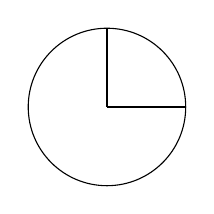
\begin{tikzpicture}
\draw (0,0) -- (1,0) ;
\draw (0,0) -- (0,1) ;
\draw (0,0) circle (1) ;
\end{tikzpicture}

\cite{souque:tel-01247368} et \cite{ravestein:hal-01777733} nous apprenent que

\input{introduction}

\section{La morphologie}

Selon

\subsection{Visualisateur}
Représentation de

\section{La morphosyntaxe}
terminologie?

\section{Conclusion}
Le 

\bibliography{paper}

% Concerns to address later:
% * Comparison with autotunning/OpenTuner in experiments
% * Show more kernels

\end{document}
